\section{Initiative}

\textbf{Initiative Checks:} At the start of a battle, each combatant makes an initiative check. An initiative check is a Dexterity check. Each character applies his or her Dexterity modifier to the roll. Characters act in order, counting down from highest result to lowest. In every round that follows, the characters act in the same order (unless a character takes an action that results in his or her initiative changing; see Special Initiative Actions).

If two or more combatants have the same initiative check result, the combatants who are tied act in order of total initiative modifier (highest first). If there is still a tie, the tied characters should roll again to determine which one of them goes before the other.

\textbf{Flat-Footed:} At the start of a battle, before you have had a chance to act (specifically, before your first regular turn in the initiative order), you are flat-footed. You can't use your Dexterity bonus to AC (if any) while flat-footed. Barbarians and rogues have the uncanny dodge extraordinary ability, which allows them to avoid losing their Dexterity bonus to AC due to being flat-footed.

A flat-footed character can't make attacks of opportunity.

\textbf{Inaction:} Even if you can't take actions, you retain your initiative score for the duration of the encounter.

\begin{figure}[t!]
\centering
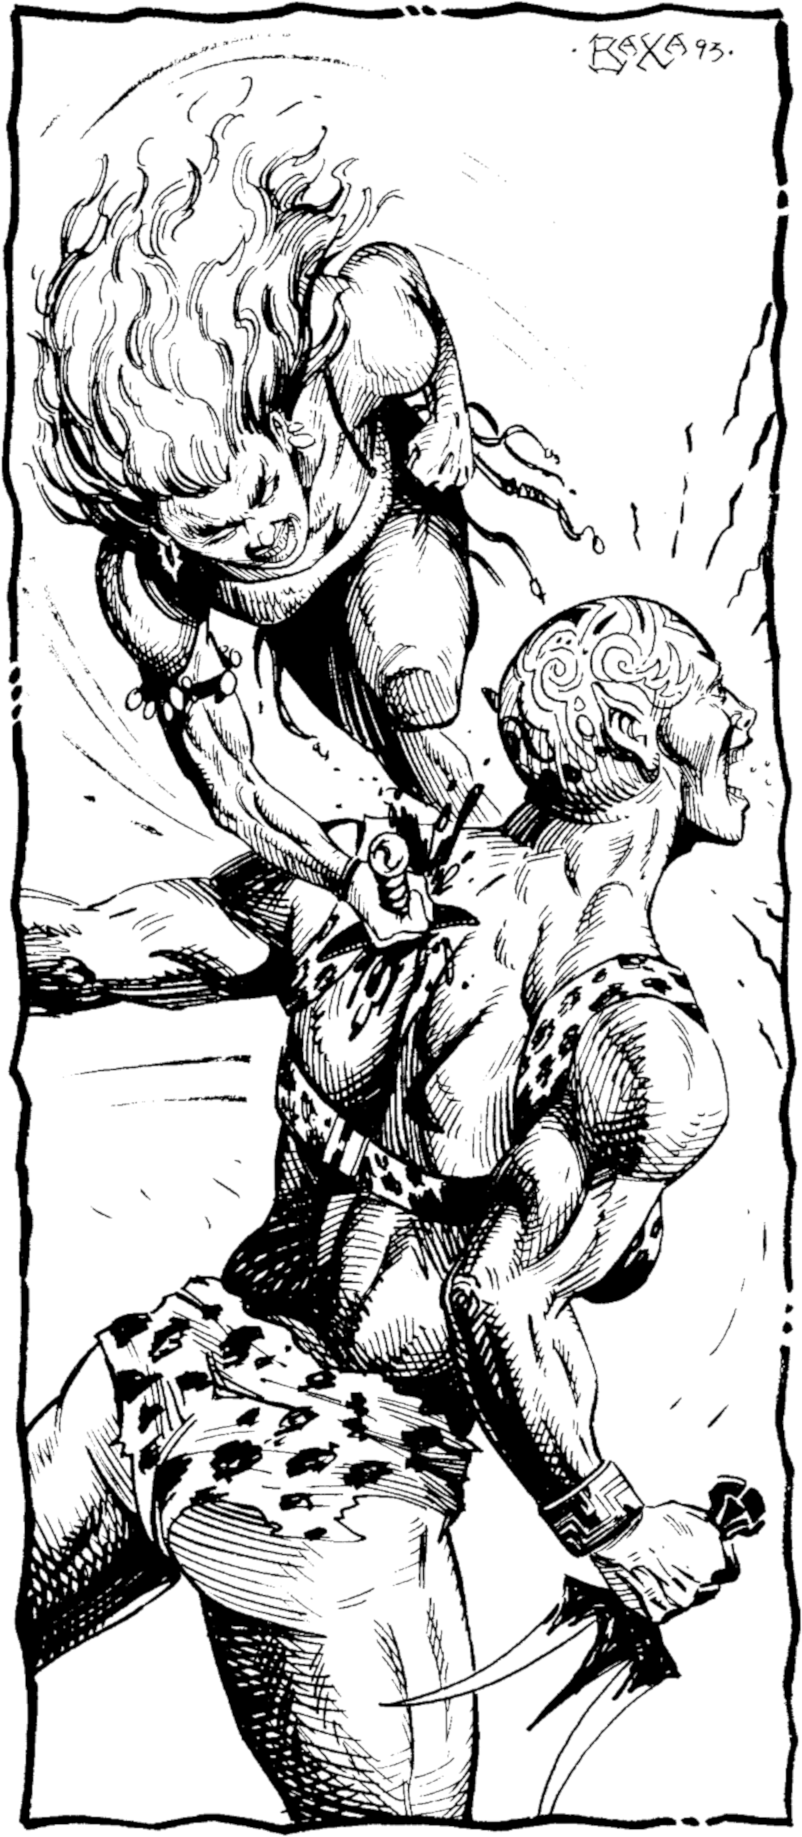
\includegraphics[width=\columnwidth-2mm]{images/killing-1.png}
\WOTC
\end{figure}

\subsection{Surprise}
When a combat starts, if you are not aware of your opponents and they are aware of you, you're surprised.

\subsubsection{Determining Awareness}
Sometimes all the combatants on a side are aware of their opponents, sometimes none are, and sometimes only some of them are. Sometimes a few combatants on each side are aware and the other combatants on each side are unaware.

Determining awareness may call for \skill{Listen} checks, \skill{Spot} checks, or other checks.

\textbf{The Surprise Round:} If some but not all of the combatants are aware of their opponents, a surprise round happens before regular rounds begin. Any combatants aware of the opponents can act in the surprise round, so they roll for initiative. In initiative order (highest to lowest), combatants who started the battle aware of their opponents each take a standard action during the surprise round. You can also take free actions during the surprise round. If no one or everyone is surprised, no surprise round occurs.

\textbf{Unaware Combatants:} Combatants who are unaware at the start of battle don't get to act in the surprise round. Unaware combatants are flat-footed because they have not acted yet, so they lose any Dexterity bonus to AC.